\documentclass[11pt,a4paper]{article}
\usepackage[T1]{fontenc}
\usepackage[utf8]{inputenc}
\usepackage{lmodern}
\usepackage{microtype}
\usepackage{amsmath,amssymb,amsthm,mathtools,bm}
\usepackage{booktabs,array,tabularx,longtable}
\usepackage{graphicx,float,caption}
\usepackage{xcolor}
\usepackage[margin=2.15cm]{geometry}
\usepackage{enumitem}
\usepackage{fancyhdr}
\usepackage[hidelinks,pdfencoding=auto]{hyperref}

\hypersetup{
  pdftitle={FIN ST233--ST247: Typed Second Operators, Nonlinear Carrier Obstructions, and Refinement Moduli},
  pdfauthor={Krzysztof Żuchowski},
  pdfsubject={Analytical, interval, and computational execution of FIN programs ST233--ST247},
  pdfkeywords={FIN, fractal information, spectral operators, selector, Blackwell experiment, continuation, quantum recovery, thermodynamics, nonlinear geometry, refinement, spectral dimension}
}

\definecolor{proved}{RGB}{20,92,48}
\definecolor{conditional}{RGB}{148,88,0}
\definecolor{blocked}{RGB}{150,28,28}
\newcommand{\Proven}{\textcolor{proved}{\textbf{[PROVEN]}}}
\newcommand{\Evidence}{\textcolor{conditional}{\textbf{[STRONG NUMERICAL EVIDENCE]}}}
\newcommand{\Conditional}{\textcolor{conditional}{\textbf{[CONDITIONAL]}}}
\newcommand{\Blocked}{\textcolor{blocked}{\textbf{[BLOCKED]}}}
\newcommand{\R}{\mathbb R}
\newcommand{\C}{\mathbb C}
\newcommand{\Tr}{\operatorname{tr}}
\newcommand{\diag}{\operatorname{diag}}
\newtheorem{theorem}{Theorem}[section]
\newtheorem{proposition}[theorem]{Proposition}
\newtheorem{corollary}[theorem]{Corollary}

\pagestyle{fancy}
\fancyhf{}
\lhead{FIN ST233--ST247}
\rhead{Release 10.73}
\cfoot{\thepage}
\setlength{\headheight}{14pt}
\setlist[itemize]{leftmargin=1.3em,itemsep=2pt,topsep=3pt}
\setlist[enumerate]{leftmargin=1.5em,itemsep=2pt,topsep=3pt}
\sloppy

\begin{document}
\hypersetup{pageanchor=false}

\begin{titlepage}
\centering
\vspace*{1.0cm}
{\Large Fractal Information Theory Project\par}
\vspace{0.9cm}
{\huge\bfseries FIN ST233--ST247\par}
\vspace{0.4cm}
{\LARGE Typed Second Operators, Nonlinear Carrier Obstructions,\par}
{\LARGE and Refinement Moduli\par}
\vspace{1.0cm}
{\large Analytical, interval, and computational research report\par}
\vfill
{\Large Krzysztof \.{Z}uchowski\par}
\vspace{0.2cm}
{\large Independent Researcher --- Fractal Information Theory Project\par}
{\large ORCID: 0009-0002-0909-3613\par}
\vspace{0.8cm}
{\large August 12, 2026\par}
\vspace{0.3cm}
{\large Release 10.73\par}
\vfill
\begin{minipage}{0.92\textwidth}
\small
\textbf{Repository snapshot.} The audited tracked base is commit
\texttt{10d0ccc19ac7b9101c7d382dd0859b352cec802f}. The working tree contains
uncommitted and untracked research artifacts. Reproduction therefore depends on the
source-packet hashes in the accompanying SHA-256 manifest, not on the tracked commit alone.

\medskip
\textbf{License.} CC BY 4.0. \quad \textbf{Language.} English. \quad
\textbf{Resource type.} Preprint and executable reproducibility package.
\end{minipage}
\end{titlepage}
\hypersetup{pageanchor=true}
\pagenumbering{roman}

\begin{abstract}
Programs ST233--ST247 execute the next local analytical and computational research batch
after the single-generator obstruction of ST218--ST232. The principal positive result is
that a genuine noncommuting second operator can be constructed in a typed way from a
vertex state: $\rho\mapsto M_\rho=\diag\rho$. For a localized strict heat state,
$[A,M_\rho]\ne0$, and layer order becomes observable. The equally important negative
result is that localization and orientation are then carried by the conditioning state;
they are not generated by the fully symmetric operator $A$ alone.

The batch also proves twelve separated likelihood-ratio classes for two adjacent strict
heat preparations by outward interval arithmetic; certifies a bounded two-step segment on
all sixty signed continuation branches; gives a rational primal--dual optimum $189/500$
for a nonunital negative-orientation qubit channel; and proves a unique continuous
minimum-entropy-production selector trajectory inside a declared two-state control model. A concrete
nonlinear coordinate change falsifies the ordinary twelfth-response ratio as a natural
nonlinear-carrier invariant and identifies a connection or jet splitting as the missing
geometric object.

At the refinement level, every self-adjoint exact extension relative to an isometry $R$ is
classified as $RAR^*\oplus B$. This turns the previous one-parameter ambiguity into a
high-dimensional moduli cone: already a two-child real symmetric refinement has 78 free
complement parameters. Repeated spectral-dimension flows consequently depend on unsourced
fiber rates and possess a scale orbit. One HMM Chernoff optimizer is only strong numerical
evidence, not an interval theorem. No strict source for the localized state, canonical
selector or connection, dimensional scale, spacetime, external record, legacy-to-strict
completion, Standard Model, gravity, or Theory-of-Everything closure is claimed.
\end{abstract}

\tableofcontents
\newpage
\pagenumbering{arabic}

\section{Executive conclusions}

The batch closes five questions and sharpens four obstructions.

\begin{enumerate}
\item A second noncommuting operator exists naturally \emph{conditional on a state}:
\[
\rho\in\Delta_{11}\longmapsto M_\rho=\diag(\rho),\qquad [A,M_\rho]\ne0.
\]
This is a typed construction, not an arbitrary matrix insertion.
\item The same construction does not solve the selector problem. The state $\rho$ carries
the symmetry breaking. A uniform condition retains $D_{12}$, an even localized condition
retains a reflection, and a chiral condition has trivial stabilizer.
\item The ordinary twelfth response is natural under linear carrier changes but not under
nonlinear charts. A connection is necessary for a covariant completion.
\item Exact coarse diffusion geometry admits an enormous family of self-adjoint
refinements. Geometry preservation alone cannot select a unique deeper layer.
\item The refinement heat trace produces calculable spectral-dimension profiles, but their
shape and scale depend on free fiber rates. They do not generate metres, seconds, or a
Planck scale.
\end{enumerate}

The deepest surviving interpretation is therefore operational and relational rather than
ontologically complete:
\[
\boxed{\text{symmetric spectral generator}+\text{typed state}
\;\Longrightarrow\;\text{ordered observable layers},}
\]
while the provenance of the state and the choice of refinement remain independent data.

\section{Scope, kernel split, and proof labels}

The strict working object is the frozen twelve-vertex graph Laplacian
\[
A=sI-W,\qquad W_{xx}=0,\qquad
W_{xy}=K_{\rm strict}(d(x,y))\quad(x\ne y),
\]
with $A\bm1=0$ and $A\succeq0$. The diagonal condition is essential: the quoted row sum
$s$ belongs to the off-diagonal weight matrix. The historical ontological kernel
$K_{\rm legacy,ont}$ remains an intermediate bridge kernel. It is not identified silently
with $K_{\rm strict}$, and no legacy physical-role formula is transferred here.

The project ontology treats the nadsoliton as primordial fractal information in a solitonic
state, with no separate informational substrate beneath it. This report tests mathematical
consequences of the frozen operator only; it does not convert that ontology into a physical
theorem.

\begin{itemize}
\item \Proven{} denotes an exact deduction or an outward finite certificate within stated
premises.
\item \Evidence{} denotes reproducible numerical evidence without a complete outward or
exact certificate.
\item \Conditional{} denotes a theorem after introducing the named state, control,
channel, connection, bath, or refinement isometry.
\item \Blocked{} denotes a required external or ungenerated object.
\end{itemize}

\section{Program ledger}

\small
\begin{longtable}{@{}>{\bfseries}p{0.07\textwidth}p{0.24\textwidth}p{0.31\textwidth}p{0.21\textwidth}@{}}
\toprule
Program & Object & Result & Boundary\\
\midrule
\endhead
ST233 & Typed second operator & \Conditional{} noncommutation and order sensitivity & Localized state is supplied\\
ST234 & Blackwell classes & \Proven{} 12 disjoint ratio intervals & Two preparations and time supplied\\
ST235 & Conditioned noise & \Proven{} stabilizer/resource theorem & Does not source the condition\\
ST236 & Branch graph & \Proven{} 120 local boxes, 30 finite components & Two steps per signed seed only\\
ST237 & Nonunital recovery & \Proven{} global CPTP optimum $189/500$ & Pauli-plus-replacer channel\\
ST238 & Continuous selector & \Proven{} unique optimum and interval cost & Two-state bath/control model supplied\\
ST239 & Nonlinear carrier & \Proven{} counterexample; \Conditional{} covariant repair & Connection is not derived\\
ST240 & Nuisance subdivision & \Proven{} 512/512 child boxes & Stratified sample, not full cube\\
ST241 & Correlated minimax & \Conditional{} sharp LAN constants & Asymptotic local experiment\\
ST242 & Clifford polar factor & \Proven{} unique fixed-$X$ solution & Joint-factor uniqueness open\\
ST243 & HMM Chernoff & \Evidence{} optimizer near $0.5022593$ & No outward sum certificate\\
ST244 & Reset ledger & \Proven{} SWAP bookkeeping and recycling bound & Blank and Hamiltonian supplied\\
ST245 & Refinement moduli & \Proven{} complete self-adjoint block classification & Local graph constraints open\\
ST246 & Spectral dimension & \Proven{} heat-trace formula; computed atlases & Fiber rates and scale unsourced\\
ST247 & External evidence & \Blocked{} & No independently registered events\\
\bottomrule
\end{longtable}
\normalsize

\section{ST233--ST235: the second operator and the selector resource}

\subsection{A state-typed noncommuting operator}

Let $\rho$ be a probability state on the twelve vertices and define the multiplication
operator
\[
M_\rho f(x)=\rho_x f(x).
\]
For $g\in D_{12}$,
\[
M_{g\rho}=gM_\rho g^{-1},
\]
so the construction is equivariant and correctly typed. Choosing
\[
\rho=e^{-0.7A}\delta_0
\]
gives a strictly positive state with numerical minimum $0.01662699154$ and
\[
\|[A,M_\rho]\|_F=0.2651939971.
\]
For comparison, $M_{\bm1/12}$ is scalar and commutes exactly with $A$.

\begin{proposition}[Order becomes observable]
For $h>0$ define
\[
S_{AB}(h)=e^{-hA}e^{-hM_\rho},\qquad
S_{BA}(h)=e^{-hM_\rho}e^{-hA}.
\]
If $[A,M_\rho]\ne0$, then the schedules differ. Moreover,
\[
\frac{S_{AB}(h)-S_{BA}(h)}{h^2}\longrightarrow [M_\rho,A]
\quad(h\downarrow0).
\]
\end{proposition}

The computed schedule difference decreases quadratically and the scaled value approaches
the commutator norm. Thus the state multiplier supplies exactly the kind of second algebra
that ST218 proved impossible inside the single-$A$ functional calculus.

\begin{figure}[H]
\centering
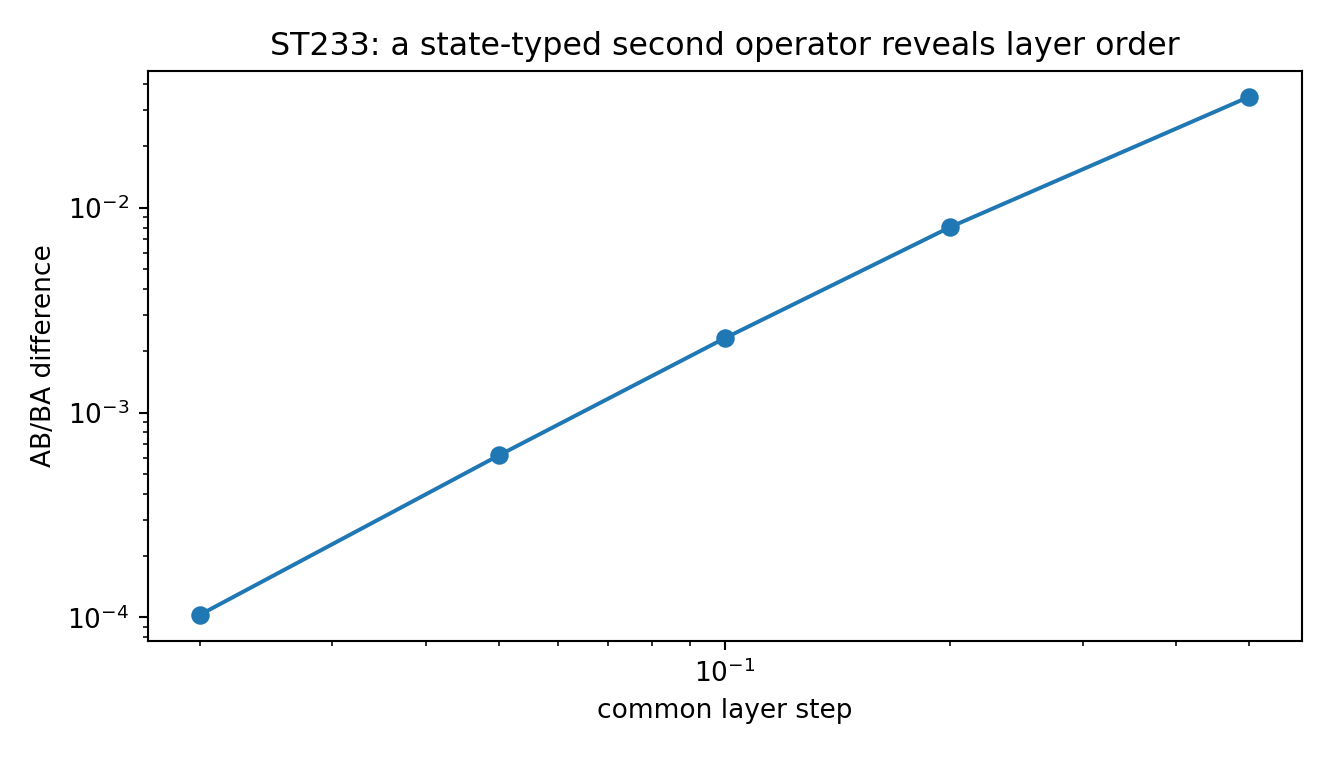
\includegraphics[width=.78\textwidth]{FIN_ST233_ST247_Figures/st233_layer_order.png}
\caption{ST233: order sensitivity produced by the state-typed multiplication operator.}
\end{figure}

\subsection{Twelve interval-separated likelihood-ratio classes}

ST234 considers the two preparations $\delta_0$ and $\delta_1$, the vertex measurement,
and $e^{-0.7A}$. Each heat entry is evaluated by interval Fourier functional calculus over
the complete frozen strict-entry enclosure. All entries remain positive. The twelve
likelihood-ratio intervals are pairwise disjoint, with minimum adjacent gap
\[
0.02428674898.
\]
For a binary experiment, outcomes with identical likelihood ratio are precisely the atoms
of the minimal sufficient partition. Hence this declared experiment has twelve atoms
throughout the supplied strict enclosure.

\begin{figure}[H]
\centering
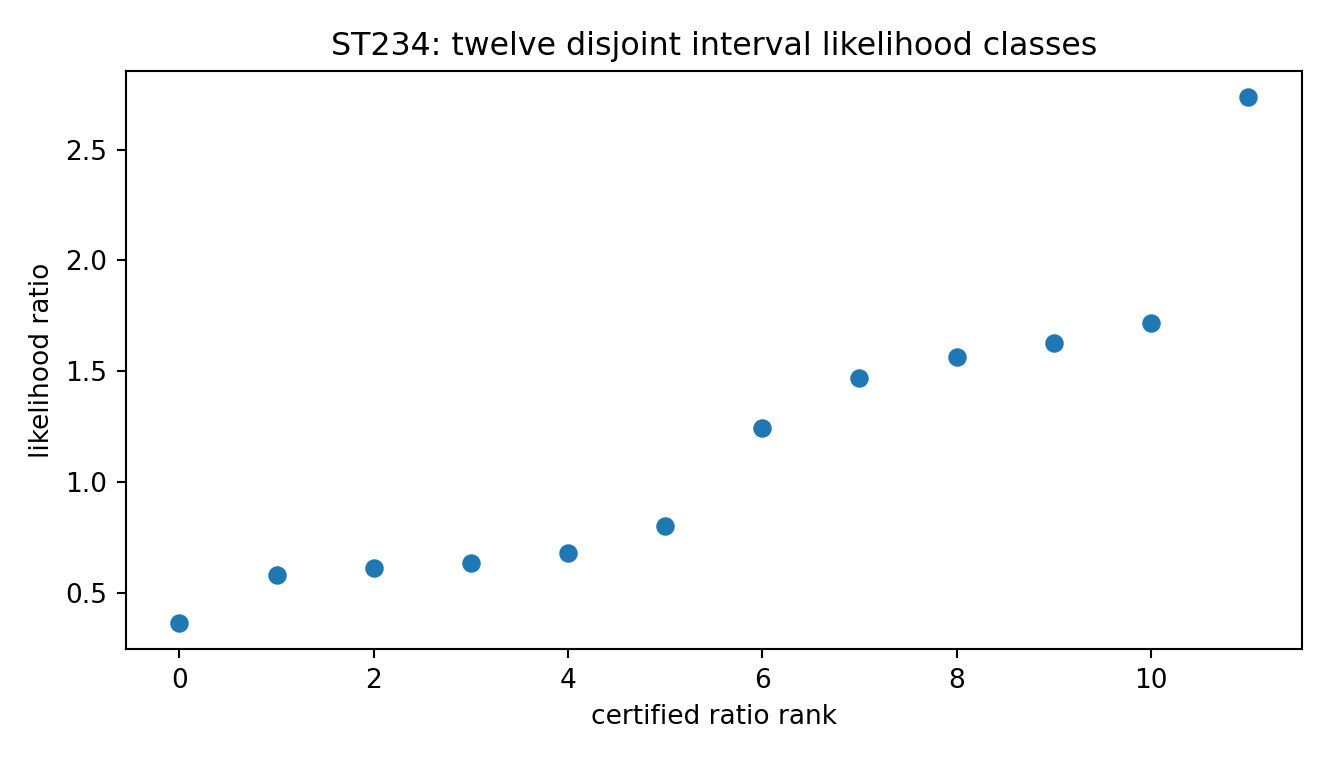
\includegraphics[width=.80\textwidth]{FIN_ST233_ST247_Figures/st234_interval_classes.png}
\caption{ST234: outward likelihood-ratio intervals, ordered by value. Error bars are much
smaller than the plotted symbols.}
\end{figure}

\subsection{The stabilizer theorem}

Let an equivariant conditional law satisfy
\[
K(g\rho,gE)=K(\rho,E).
\]
After fixing $\rho$, the output can distinguish only orbits of its stabilizer
$G_\rho$. The complete finite calculation gives
\[
\begin{array}{c|cccc}
\rho & \bm1/12 & \delta_0 & e^{-0.7A}\delta_0 & \text{chiral localized}\\ \hline
|G_\rho| &24&2&2&1\\
\#\text{ vertex orbits}&1&7&7&12.
\end{array}
\]
An even localized state selects a vertex but not an orientation. A chiral state supplies
both. This is the precise resolution of the apparent paradox: conditioning permits
selection, but selection information is in the condition.

\begin{figure}[H]
\centering
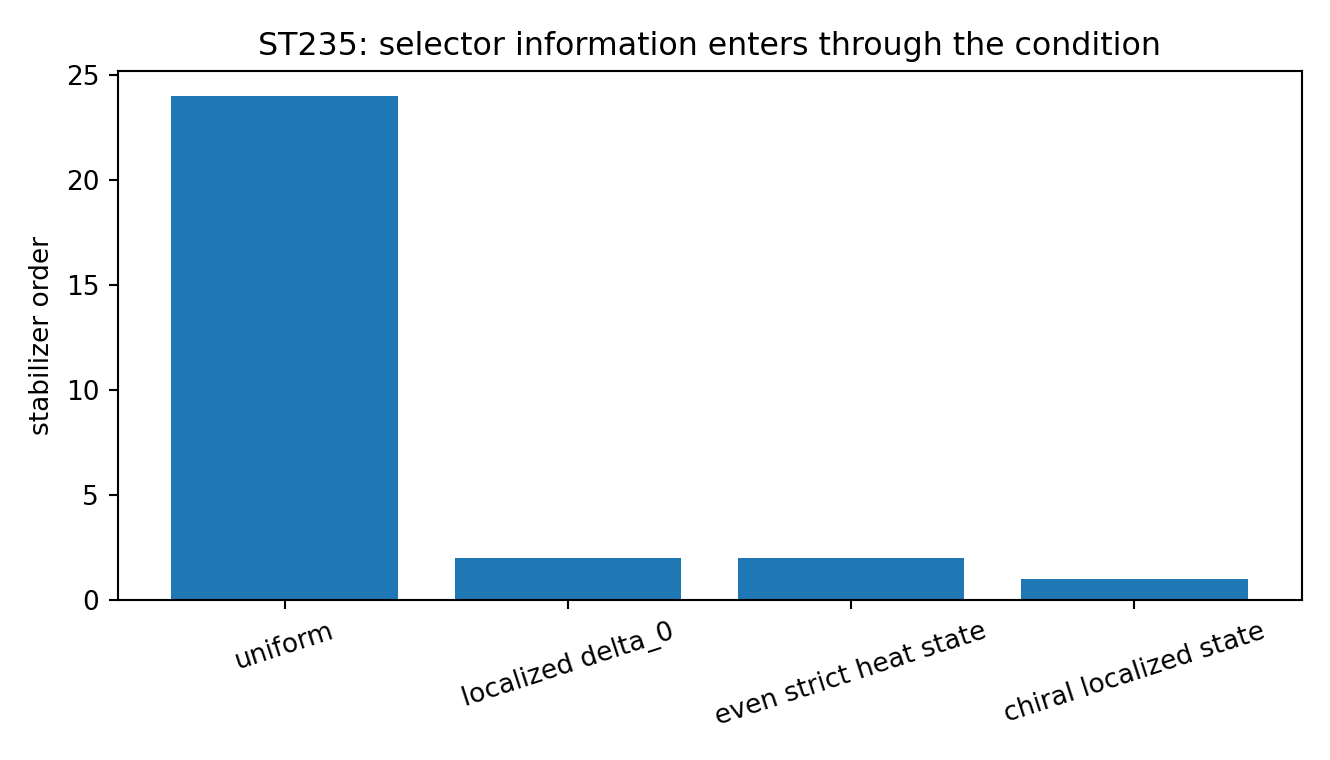
\includegraphics[width=.78\textwidth]{FIN_ST233_ST247_Figures/st235_stabilizers.png}
\caption{ST235: residual symmetry and distinguishable vertex orbits.}
\end{figure}

\section{ST236: bounded all-branch continuation}

The sixty signed seeds inherited from the exact fold campaign were advanced by two
pseudo-arclength steps each. Every one of the 120 stationary points has an outward
Krawczyk inclusion. The minimum seven-row rank margin is
$2.61998\times10^{-3}$. Opposite signed seeds with the same amplitude and Fourier mode
meet at one of thirty exact uniform folds. All boxes from different fold pairs are
disjoint, with minimum coordinate clearance $0.00606308$.

\begin{theorem}[Finite certified incidence graph]
The declared set of 120 local boxes and thirty exact fold links has thirty connected
components. This statement is exact for the finite graph.
\end{theorem}

It is not a theorem about untraced branch segments. A collision, reconnection, or secondary
bifurcation outside the two-step windows remains possible.

\begin{figure}[H]
\centering
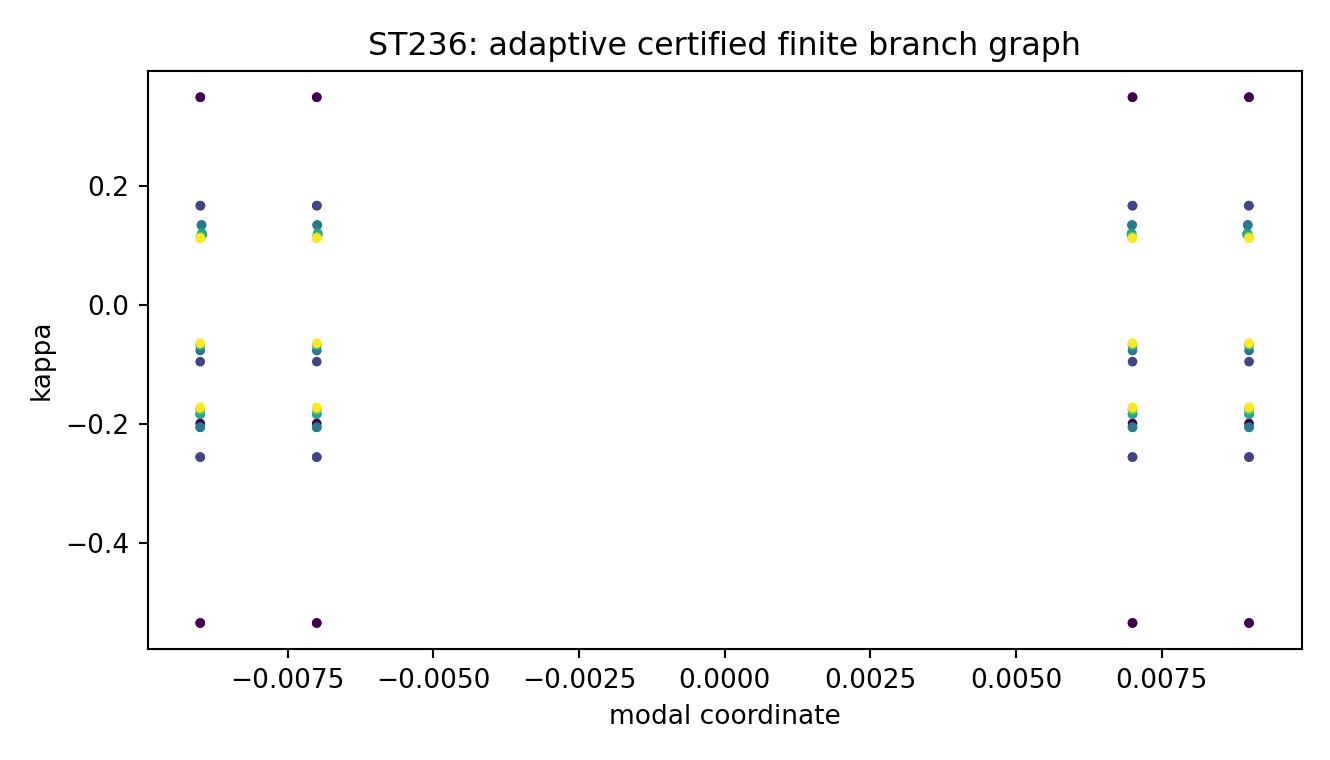
\includegraphics[width=.85\textwidth]{FIN_ST233_ST247_Figures/st236_branch_graph.png}
\caption{ST236: bounded certified continuation issued from all signed fold seeds.}
\end{figure}

\section{ST237: exact recovery of a nonunital negative-orientation channel}

Consider
\[
\mathcal N=\frac45\mathcal P+\frac15\mathcal R_0,
\qquad \mathcal R_0(\rho)=|0\rangle\!\langle0|\Tr\rho,
\]
where the Pauli probabilities are
\[
(p_I,p_X,p_Y,p_Z)=\left(\frac2{25},\frac{41}{100},
\frac{29}{100},\frac{11}{50}\right).
\]
Its Bloch linear part has determinant $-0.00106496$ and translation $(0,0,1/5)$, so the
example is both negative-orientation and genuinely nonunital.

\begin{theorem}[Global CPTP recovery optimum]
For every trace-preserving recovery $\mathcal R$,
\[
F_e(\mathcal R\circ\mathcal N)\le
\frac45\frac{41}{100}+\frac15\frac14=\frac{189}{500}.
\]
The unitary $X$ recovery attains the bound. A rational Choi primal and a dual matrix have
equal value; the computed dual slack eigenvalues are
\[
(0,0.048,0.076,0.132)
\]
up to $2.1\times10^{-17}$ floating replay error.
\end{theorem}

The theorem is global over all CPTP recoveries for this channel family, not for arbitrary
affine qubit channels.

\section{ST238 and ST244: what selection and reset cost}

\subsection{A verified continuous selector path}

The declared two-state reduction obeys
\[
\dot x=\pi-x,\qquad 0\le \pi\le1,
\]
and uses the Markov entropy-production density
\[
L(x,\pi)=(\pi-x)\bigl(\operatorname{logit}\pi-
\operatorname{logit}x\bigr).
\]
For $x(0)=1/12$, $x(4)=0.6$, the unique continuous optimum has first integral
\[
C=\frac{\dot x^2}{\pi(1-\pi)},
\qquad
\pi(x,C)=\frac{2x+C+\sqrt{C^2+4Cx(1-x)}}{2(1+C)}.
\]
Outward quadrature proves
\[
C\in[0.0744,0.0747],\qquad
\Sigma\in[0.3176910887,0.3191979592].
\]
The travel-time interval at $C=0.0744$ lies strictly above four, while the interval at
$C=0.0747$ lies strictly below four.

\begin{figure}[H]
\centering
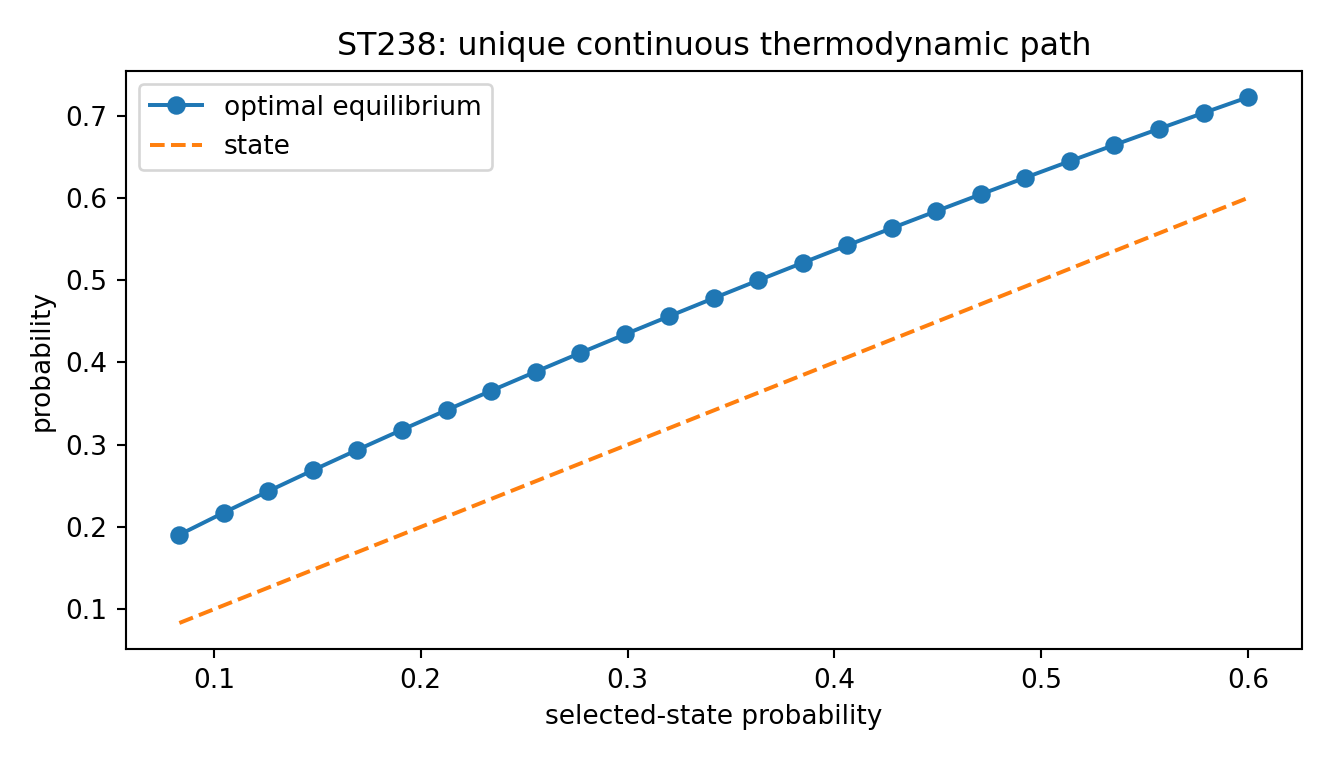
\includegraphics[width=.83\textwidth]{FIN_ST233_ST247_Figures/st238_continuous_control.png}
\caption{ST238: optimal equilibrium control and the induced monotone state trajectory.}
\end{figure}

This prices a selector trajectory only after supplying the bath, preferred vertex,
two-state reduction, maximum rate, endpoints, and dimensionless time. It does not generate
the selector or convert the cost into joules.

\subsection{Reset moves information; recycling pays}

For identical register Hamiltonians, the global SWAP implements
\[
\rho\otimes|0\rangle\!\langle0|
\longmapsto |0\rangle\!\langle0|\otimes\rho.
\]
The joint spectrum, entropy, and total energy are unchanged. Hence the reversible logical
step has $\Delta F_{\rm total}=0$: information is transferred to the ancilla, not erased.
Restoring the blank requires at least
\[
W\ge F_\beta(|0\rangle\!\langle0|)-F_\beta(\rho).
\]
For a degenerate Hamiltonian and $\beta=1$, this is $S(\rho)$ and reaches $\log16$ for the
maximally mixed input. The controller work and finite-time friction remain unpriced.

\section{ST239: a nonlinear-carrier no-go and the missing connection}

Take
\[
V(x)=\frac a2x^2+\frac g{12}x^{12},\qquad x=y+cy^6.
\]
At the origin the Hessian and tangent scale are unchanged, yet
\[
\frac{D^{12}_yV}{11!}=g+6ac^2.
\]
For $(a,g,c)=(1.7,0.4,0.3)$, the ordinary normalized response changes from
$0.01657168$ to $0.05460368$. Thus ordinary higher derivatives do not define a nonlinear
carrier-natural tensor.

\begin{theorem}[Necessary geometric completion]
To transport the twelfth response naturally under nonlinear carrier charts, one must add a
connection or an equivalent jet splitting. Conditional on a transported connection,
\[
\mathcal I_{12}^{\nabla}=
\frac{(\nabla^{12}V)(v^{\otimes12})}
{11!\,[(\nabla^2V)(v,v)]^6}
\]
is a scalar under chart change.
\end{theorem}

The connection is a newly identified missing object; no canonical strict source for it is
known.

\section{ST240--ST243: validation boundaries and statistical inference}

\subsection{Certificate failure is not root loss}

At global nuisance halfwidth $5\times10^{-4}$, 64 deterministic cells selected from four
strata per coordinate all fail the coarse Krawczyk test with local halfwidth
$2.0833\times10^{-5}$. Splitting each into eight children reduces the local halfwidth to
$1.0417\times10^{-5}$; all 512 children pass, with minimum margin $0.001779$.

Therefore these are certificate-resolution failures, not root-loss events in those boxes.
The 64 parents do not cover the full cube, and the result must not be reported as a full
$5\times10^{-4}$ continuation theorem.

\subsection{Sharp modal minimax constants}

Within the declared regular six-parameter local experiment, local asymptotic normality
gives
\[
R_{\rm trace}\sim\frac{\Tr(I^{-1})}{n},\qquad
R_{\rm worst\ mode}\sim\frac{\max_k I_k^{-1}}{n}.
\]
For exchangeable clusters of size $20$ and intracluster correlation $0.05$, both constants
are multiplied by
\[
1+(20-1)0.05=1.95.
\]
This is an asymptotic conditional theorem, not a finite-sample detector guarantee.

\begin{figure}[H]
\centering
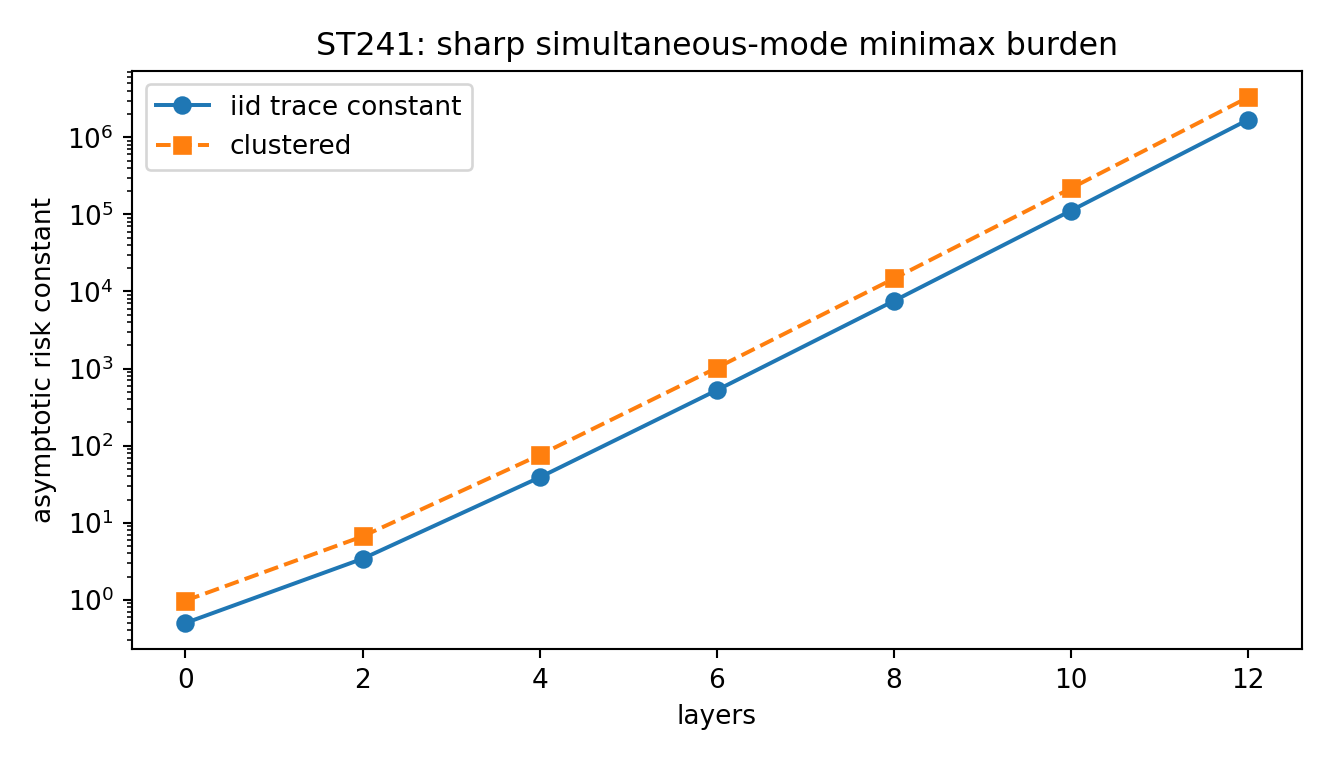
\includegraphics[width=.82\textwidth]{FIN_ST233_ST247_Figures/st241_minimax_constants.png}
\caption{ST241: trace-risk constants and their cluster inflation across developed layers.}
\end{figure}

\subsection{Higher-dimensional fixed-factor Clifford projection}

Fix the balanced involution $X=\diag(I_n,-I_n)$. Every Hermitian involution
anticommuting with $X$ has form
\[
Z(U)=\begin{pmatrix}0&U\\U^*&0\end{pmatrix},\qquad U\in U(n).
\]
Projecting a target first to its $X$-odd block $C$ reduces the nearest-factor problem to
unitary Procrustes. If $C$ is invertible, its polar unitary
$U=C(C^*C)^{-1/2}$ is the unique global minimizer. Numerical replays for $n=2,3,4$ have
unitarity and involution errors below $2.1\times10^{-15}$. This theorem fixes $X$ first;
simultaneous global uniqueness of both factors is not implied.

\subsection{Chernoff optimization: intentionally not promoted}

For all $2^{16}=65{,}536$ records of the supplied binary HMM, long-double summation gives
\[
s_*\approx0.50225930327,
\quad
Z_{16}(s_*)\approx6.69672763505\times10^{-6}.
\]
The derivative changes sign across $[0.5022593,0.5022594]$, and the optimized coefficient
is smaller than the $s=1/2$ coefficient $6.69881023894\times10^{-6}$. Exact strict
convexity of $Z_{16}$ proves that a true derivative zero is unique. However, the endpoint
sums were not enclosed by outward interval arithmetic. The location and the induced
asymptotic candidate bracket $[0.68990,0.81987]$ are therefore \Evidence{}, not a proof
certificate.

\section{ST245--ST246: complete refinement moduli and spectral dimension}

\subsection{The complete self-adjoint classification}

Let $R:\R^{12}\to\R^{12q}$ be an isometry and suppose
\[
\widetilde A R=RA,\qquad \widetilde A=\widetilde A^*.
\]
Self-adjointness makes $\operatorname{Ran}R$ reducing. Hence
\[
\boxed{\widetilde A=RAR^*\oplus B
\quad\text{on }\operatorname{Ran}R\oplus(\operatorname{Ran}R)^\perp.}
\]
Conversely every self-adjoint $B$ yields exact functional-calculus intertwining, and
$B\succeq0$ preserves positivity. With $m=12(q-1)$, the real symmetric moduli dimension is
$m(m+1)/2$:
\[
\begin{array}{c|rrrr}
q&2&3&4&5\\ \hline
m&12&24&36&48\\
\dim\operatorname{Sym}(m)&78&300&666&1176.
\end{array}
\]
Three independent $q=3$ replays preserve generator intertwining and coarse heat distances
to errors below $10^{-14}$. The earlier one-rate Kronecker refinement is only a tiny slice
of this cone.

\subsection{Exact repeated-refinement heat formula}

For two-state fiber gaps $\mu_j$, heat traces multiply under Kronecker sums. Therefore
\[
d_s(t)=2t\langle\lambda\rangle_t+
\sum_j\frac{4\mu_jt}{e^{2\mu_jt}+1}.
\]
Constant rates create a growing intermediate peak; geometrically separated rates create
staged contributions. Neither is selected by coarse FIN geometry. Moreover,
\[
\mu_j\mapsto c\mu_j,qquad t\mapsto t/c
\]
leaves every fiber contribution invariant. Frequency and spectral flow supply
dimensionless phase/time ratios only; they do not select seconds or lengths.

\begin{figure}[H]
\centering
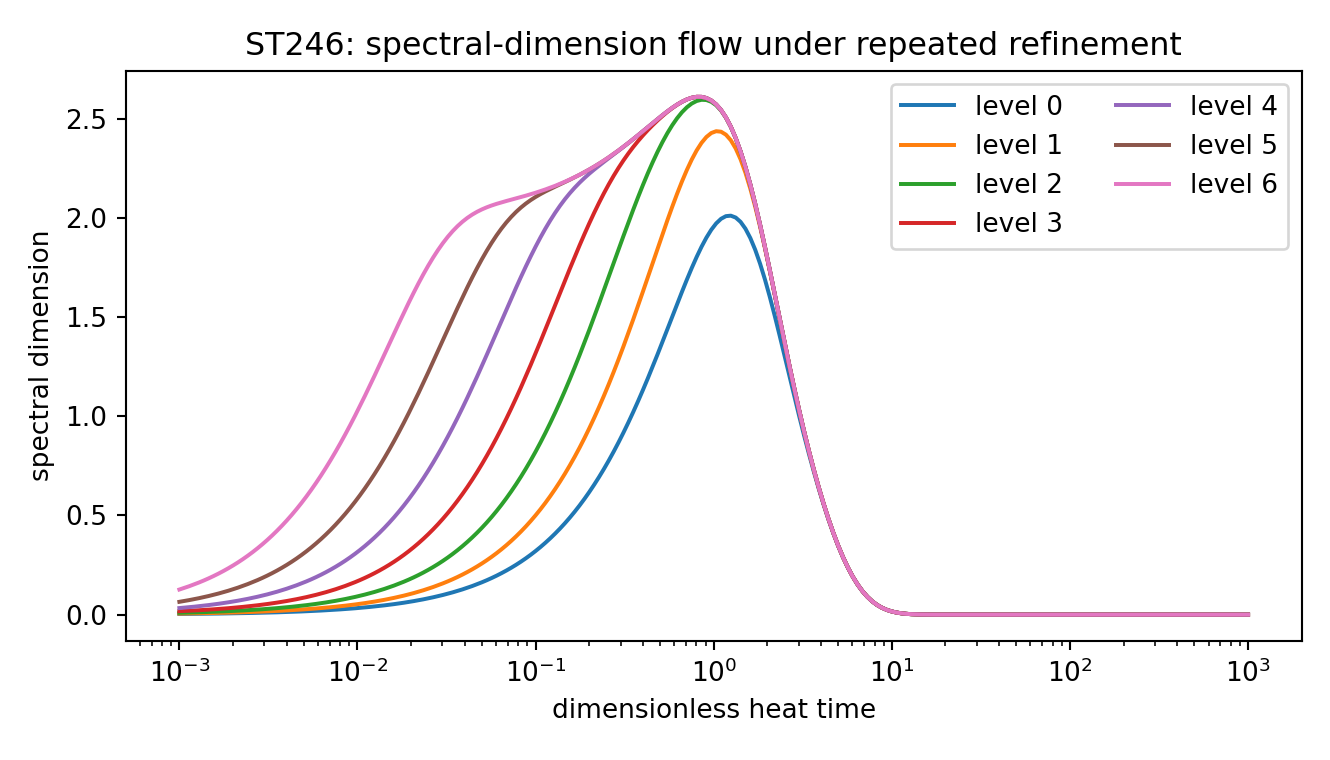
\includegraphics[width=.86\textwidth]{FIN_ST233_ST247_Figures/st246_spectral_dimension.png}
\caption{ST246: spectral-dimension flows for constant and geometric fiber-rate choices.}
\end{figure}

\section{Falsification ledger}

\begin{longtable}{@{}p{0.29\textwidth}p{0.32\textwidth}p{0.30\textwidth}@{}}
\toprule
Candidate claim & Falsification or surviving result & Epistemic consequence\\
\midrule
One symmetric operator contains layer order & Every $f(A)$ commutes; ST233 needs $M_\rho$ & Second typed object is necessary\\
Conditioned noise generates a selector & Stabilizer information is inherited from $\rho$ & State provenance remains open\\
Linear response naturality extends nonlinearly & Explicit $x=y+cy^6$ counterexample & Connection/jet splitting required\\
Coarse certificate failure signals root loss & 512 child boxes all pass & Numerical method failure separated from ontology\\
HMM optimizer is interval certified & Endpoint sums are long-double, not outward & Demoted to strong numerical evidence\\
Exact diffusion refinement is essentially unique & Full $RAR^*\oplus B$ classification & Large nonuniqueness moduli proved\\
Repeated refinement generates physical scale & Fiber rates free; simultaneous scale orbit & No seconds, lengths, or Planck scale\\
Local computation can create external evidence & No registered laboratory record exists & ST247 remains blocked\\
\bottomrule
\end{longtable}

\section{Relation to FIN ontology and the projection intuition}

The results are compatible with an information-first interpretation only in a limited,
mathematical sense. A single spectral generator supports several functional channels, and
a state-typed multiplication algebra makes order and preparation operationally visible.
Refinement can hide arbitrary complement dynamics from all coarse observables. These facts
make a ``deeper state projected to a coarser observation'' architecture mathematically
possible.

They do not prove that the observed universe is such a projection. In fact, ST245 makes the
inverse problem harder: infinitely many deeper operators yield exactly the same coarse
heat geometry. To turn layered fractal compression into physics, one needs a rule that
selects $R$, $B$, a state, an instrument, a clock, and dimensional calibration, followed by
observables that distinguish the selected refinement from alternatives. Seeing lower
scales through fractal layers is therefore a research hypothesis, not a consequence of the
current strict kernel.

Likewise, symmetry is a reservoir of equivalent possibilities, not positive feedback by
itself. Positive feedback requires a dynamical gain or instability. A state with reduced
stabilizer can select and amplify one branch, but ST235 proves that the asymmetry is then
carried by that state unless a strict internal source is found. QW-2191 remains open.

\section{Recommended programs ST248--ST262}

\begin{enumerate}
\item[\textbf{ST248}.] Search for a strict source of the preparation entering
$M_\rho$, or prove a preparation-source no-go.
\item[\textbf{ST249}.] Classify all $D_{12}$-natural typed second operators in the vertex
multiplication and commutant algebras, with their minimal conditioning data.
\item[\textbf{ST250}.] Extend the branch graph only until an interval-certified collision,
closure, or declared global resource stop.
\item[\textbf{ST251}.] Solve one generic rational affine-qubit recovery instance outside
the Pauli-plus-replacer symmetry.
\item[\textbf{ST252}.] Add endpoint preparation and finite-rate actuator costs to the
continuous selector optimum.
\item[\textbf{ST253}.] Search for a canonical connection from strict response data and
apply the ST239 obstruction test.
\item[\textbf{ST254}.] Complete the halfwidth-$0.0005$ nuisance shell by adaptive covering,
or stop at a predeclared resource boundary.
\item[\textbf{ST255}.] Construct finite-sample estimators approaching the ST241 correlated
minimax constants.
\item[\textbf{ST256}.] Prove or refute global joint higher-dimensional Clifford-factor
uniqueness under two simultaneous spectral gaps.
\item[\textbf{ST257}.] Replace the block Chernoff comparison by a certified
belief-transfer spectral-radius enclosure.
\item[\textbf{ST258}.] Include pulse-controller work and finite-temperature blank
preparation in reset bookkeeping.
\item[\textbf{ST259}.] Intersect the ST245 moduli cone with graph-Laplacian positivity,
locality, and declared symmetry constraints.
\item[\textbf{ST260}.] Test whether any internally selected fiber-rate distribution yields
a stable spectral-dimension plateau.
\item[\textbf{ST261}.] Derive operational observables capable of distinguishing two
members of the refinement moduli cone.
\item[\textbf{ST262}.] Resume external validation only after independently registered
laboratory events, calibration hashes, and custody records exist.
\end{enumerate}

The top priority is ST248. Without a source for the state, the newly constructed second
operator is an operational completion, not a strict-core derivation. ST253 and ST259 are
the next most informative obstruction tests: they ask whether the new connection and the
large refinement cone can be reduced by already available strict data.

\section{Reproducibility}

The executable source is \texttt{fin\_st233\_st247\_research.py}. It writes one aggregate
JSON file, one CSV ledger, fifteen per-program JSON packets, and seven figures. The
lightweight independent replay \texttt{test\_fin\_st233\_st247.py} checks packet hashes,
live noncommutation, exact rational identities, interval ordering, all stored continuation
inclusions, status discipline, and the epistemic boundary. The SHA-256 manifest fixes the
release byte-for-byte.

The numerical environment recorded in the aggregate JSON includes Python, NumPy, SciPy,
and SymPy versions. ST234, ST236, ST238, and ST240 use outward interval/Krawczyk logic;
ST243 explicitly does not and is labeled accordingly. Random demonstrations use the fixed
seed \texttt{20260812}.

\section{Final conclusion}

The new research does not close FIN as physics. It does identify two missing theoretical
objects more precisely than before:
\begin{align*}
&\boxed{\text{a sourced state/preparation for the second algebra}},\\
&\boxed{\text{a canonical connection for nonlinear carrier response}}.
\end{align*}
It also proves that a third hoped-for shortcut fails: exact preservation of coarse
diffusion geometry cannot choose a unique fractal refinement because the complement
generator $B$ remains free in a high-dimensional cone.

The strongest defensible present statement is this: FIN's strict operator admits a coherent
operational extension in which state, layer order, measurement discrimination, control
cost, and multiscale refinement can be treated rigorously. The same mathematics proves
that the state, nonlinear connection, dimensional scale, and deeper refinement are not yet
inevitable consequences of the strict operator. That boundary, rather than a claim of
physical closure, is the scientific result of ST233--ST247.

\end{document}
